\begin{figure}
  \centering
  \begin{tabular}{cc}
    \begin{minipage}{0.5\hsize}
      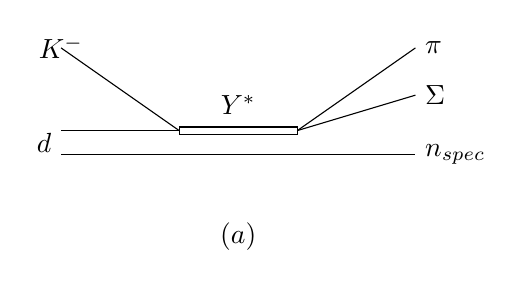
\begin{tikzpicture}[scale=1.5]
        \draw (-1.5,    0.7) node {$K^-$}--(-0.5,    0);
        \draw (-1.5,    0)--(-0.5,    0);
        \draw (-0.5, 0.03) rectangle (0.5, -0.03);
        \draw (0.0, 0.05) node [above]{$Y^*$};
        \draw (0.5, 0)--(1.5, 0.3) node [right] {$\Sigma$};
        \draw (0.5, 0)--(1.5, 0.7) node [right] {$\pi$};
        
        \draw (-1.5, -0.2)--(1.5, -0.2) node [right] {$n_{spec}$};
        \node (d) at (-1.5, -0.1) [left] {$d$};

        \draw (0, -0.7) node [below] {$(a)$};
      \end{tikzpicture}
    \end{minipage}

    \begin{minipage}{0.5\hsize}
      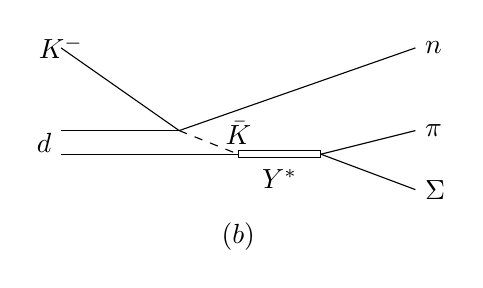
\begin{tikzpicture}[scale=1.5]
        \draw (-1.5,    0.7) node {$K^-$}--(-0.5,    0);
        \draw (-1.5,    0)--(-0.5,    0);
        \draw (-1.5, -0.2)--(0.0, -0.2);
        \node (d) at (-1.5, -0.1) [left] {$d$};
        
        \draw (-0.5, 0) -- (0.0, -0.2) [dashed];
        \node (barK) at (0.0, -0.2) [above] {$\bar{K}$};

        \draw ( -0.0, -0.23) rectangle (0.7, -0.17);
        \draw ( 0.35, -0.25) node [below] {$Y^*$};
        
        \draw ( 1.5,  -0.5) node [right] {$\Sigma$} -- (0.7, -0.2);
        \draw ( 1.5,  -0.0) node [right] {$\pi$}    -- (0.7, -0.2);
        \draw ( 1.5,  0.7) node [right] {$n$}      -- (-0.5,    0);
        \draw (0, -0.7) node [below] {$(b)$};
      \end{tikzpicture}
    \end{minipage}
  \end{tabular}
  \caption{
    This figure is a diagram of the $K^-d\rightarrow n \Sigma \pi$ reaction.
    The left figure (a) represents a one-nucleon reaction, and the right figure (b) represents a two-step reaction.    
  }
  \label{fig:kd_diag}
\end{figure}
